\documentclass[a4paper,11pt]{jsarticle}


% 数式
\usepackage{amsmath,amsfonts}
\usepackage{physics}
\usepackage{bm}
\usepackage{cases}
\usepackage{listings,jlisting}
\lstset{
  language=Python,
  basicstyle={\ttfamily},
  identifierstyle={\small},
  keywordstyle={\bfseries},
  ndkeywordstyle={\small},
  commentstyle={\small},
  stringstyle={\small\ttfamily},
  frame={tb},
  breaklines=true,
  columns=[l]{fullflexible},
  numbers=left,
  xrightmargin=0zw,
  xleftmargin=0zw,
  numberstyle={\scriptsize},
  stepnumber=1,
  numbersep=1zw,
  lineskip=-0.5ex
}

% 画像
\usepackage[dvipdfmx]{graphicx}
\usepackage[dvipdfmx]{hyperref}
\usepackage{here}


% その他
\usepackage[top=30truemm,bottom=30truemm,left=25truemm,right=25truemm]{geometry}

\begin{document}

\title{数値解析 最終レポート\\単振り子および二重振り子の運動方程式に対するRunge-Kutta法の適用}
\author{計数工学科 J4190147 小野悠太}
\date{\today}
\maketitle
\newpage
\setcounter{tocdepth}{3}
\tableofcontents
\newpage

\section{目的}
このレポートでは,二重振り子の運動方程式に対してRunge-Kutta法を適用し数値解を求め,運動を可視化したうえで系の全エネルギーがどれほどの精度で保存されるのかを確かめることを目的とする.\\
このような目的を定めた理由としては,1Aセメスターで受講した「振動波動論」で二重振り子のカオスが紹介されておりその複雑な運動に興味を持ったことや今セメスターの「数学1D」で解析力学を習い,二重振り子の運動方程式を立てやすくなったことが挙げられる.また,カオスという複雑で非周期的な運動に対しRunge-Kutta法を適用しても,期待される精度が出るのか気になったことも理由の一つである.\par
具体的な設定や実験方法については後の章で説明する.また,ここで扱う二重振り子のモデルはそれぞれの振り子の腕の先端に質点が存在するモデル(単振り子を連結したもの)とする.図のキャプションなどで現れるRK4という文字列は4段4次のRunge-Kutta法を表すものとする.

\newpage

\section{単振り子の運動}
この章では二重振り子ではなく単振り子を扱う.この運動はカオスではない.まず単振り子に対してRunge-Kutta法を適用して系のエネルギーの変化を求めることで,カオスである場合とそうでない場合の比較を可能とすることを目的としている.\\
また,今回扱う二重振り子のモデルは単振り子を2つ直列に連結したものであるから,これらの結果に類似性が見られることも期待される.

\subsection{単振り子の運動方程式}
ここでは,振り子の腕の一方が原点\(O\)に固定されており,他方の端点には質量\(m_1\)の質点が取り付けられているとする.\\
\(\theta\)は鉛直下方向と振り子の腕がなす角とし,腕の長さを\(l\)とする.
これは極めて一般的な振り子であり,その運動方程式は以下のようにあらわされる.
\begin{equation}
  \ddot{\theta} = -\dfrac{g}{l}\sin{\theta}
\end{equation}
\(\dot{\theta} = \omega\)とするとこの運動方程式は,一階の微分方程式を連立させたものとなる.
\begin{subnumcases} 
  {\label{eom:single}}
  \dot{\theta} = \omega & \\
  \dot{\omega} = -\dfrac{g}{l}\sin{\theta} &
\end{subnumcases}

\subsection{単振り子の運動方程式に対するRunge-Kutta法の適用}
以下では式(\ref{eom:single})に対してRunge-Kutta法を適用することを考える.
\begin{equation}
  f(\theta) = -\dfrac{g}{l}\sin{\theta}
\end{equation}
として,
\begin{gather}
  k_1 = f(\theta^{(m)}) \\
  n_1 = \omega^{(m)} \\
  k_2 = f\qty(\theta^{(m)}+\dfrac{n_1}{2}\Delta t) \\
  n_2 = \omega^{(m)} + \dfrac{k_1}{2}\Delta t \\
  k_3 = f\qty(\theta^{(m)}+\dfrac{n_2}{2}\Delta t) \\
  n_3 = \omega^{(m)} + \dfrac{k_2}{2}\Delta t \\
  k_4 = f\qty(\theta^{(m)} + n_3 \Delta t) \\
  n_4 = \omega^{(m)} + k_3 \Delta t
\end{gather}
と定義すると,
\begin{equation}
  \omega^{(m+1)} = \omega^{(m)} + \qty(\dfrac{1}{6}k_1+\dfrac{1}{3}k_2+\dfrac{1}{3}k_3+\dfrac{1}{6}k_4)\Delta t
\end{equation}
\begin{equation}
  \theta^{(m+1)} = \theta^{(m)} + \qty(\dfrac{1}{6}n_1+\dfrac{1}{3}n_2+\dfrac{1}{3}n_3+\dfrac{1}{6}n_4)\Delta t
\end{equation}
と表せる.\\
今回はこれをPythonにより実装し,運動の可視化およびそのエネルギー変化を可視化した.
運動の可視化のプログラムは付録中のソースコード\ref{src:RK41anim},エネルギーの時間変化のグラフを作成するプログラムはソースコード\ref{src:RK41eval2},時間幅の取り方によるエネルギーの誤差の変化を可視化するプログラムはソースコード\ref{src:RK41eval1}に示す.\\

\newpage
\subsection{結果}
\subsubsection{単振り子の運動のアニメーション}
ソースコード\ref{src:RK41anim}では長さ\(l\),質量\(m\),初角度\(\theta_0\),初角速度\(\omega_0\)がパラメータとして設定できるようになっているが,ここでは,\(l=1\),\ \(m=1\),\ \(\omega_0=0\)として運動の様子を見る.\\
このプログラムでは運動の様子をシミュレーションしたアニメーションがgifファイルとして保存できるが,このレポート上にgifを直接掲載するのは難しかったため,以下のリンク先(Google drive)に保存した.
\begin{itemize}
  \item \href{https://drive.google.com/file/d/1HEMIiebBH-CA8qKj4L7jN1CmuGO9943t/view?usp=sharing}{初角\(\dfrac{\pi}{4}\)の単振り子}
  \item \href{https://drive.google.com/file/d/1J6pF6LpVSzd1oC3yWCBBsiJDz6IESJB8/view?usp=sharing}{初角\(\dfrac{\pi}{3}\)の単振り子}
\end{itemize}
これらのアニメーションでは特に不自然に見える箇所はなく,Runge-Kutta法によって作成した単振り子の運動と人間が想像する単振り子の運動との間には大きな乖離はないと考えられる.

\subsubsection{エネルギー誤差の時間変化}
視覚的な運動が想像と一致していても,系としての構造をきちんと保っているとは限らない.\\
よって,ここではこの系に対してRunge-Kutta法を適用したときにエネルギーが時間経過とともにどのように変化しているかを観察する.\par
ソースコード\ref{src:RK41eval2}では長さ\(l\),質量\(m\),初角速度\(\omega_0\)がパラメータとして設定できるようになっているが,ここでは,\(l=1\),\ \(m=1\),\ \(\omega_0=0\)とした.\par
本来この系では運動エネルギーとポテンシャルエネルギーの和(力学的エネルギー)が保存されており,そのような結果が得られることが望ましい.
下の図\ref{fig:RK41_eval2}はソースコード\ref{src:RK41eval2}において初角度を\(\theta_0 = \dfrac{\pi}{4}\)としたものであり,縦軸に真の力学的エネルギーと計算された力学的エネルギーの差(\(E_0 - E\)),横軸に経過時間をとっている.
初期条件より\(E_0\)は負の定数であるから,このグラフからは\(E (< 0)\)が時間経過とともに小さくなっていっていることが読み取れる.\\
なお,図中の点線は\(f(t) = 3\times10^{-9}t\)の直線である.
\begin{figure}[H]
  \begin{center}
    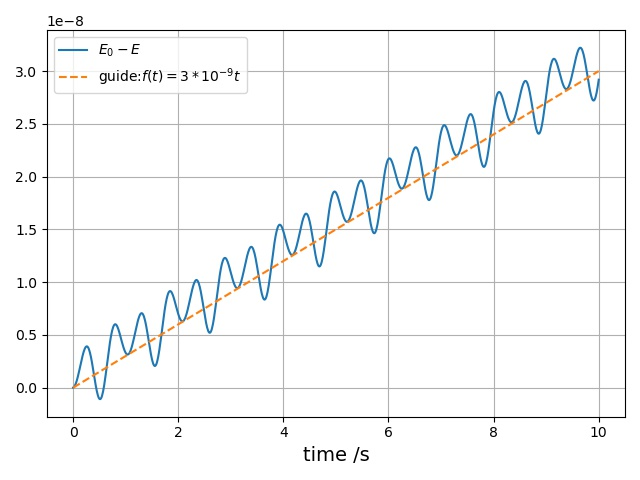
\includegraphics[scale=0.6]{figure/RK41/evaluation2/2021-2-9-223945.jpeg}
    \caption{系のエネルギー誤差の時間変化}
    \label{fig:RK41_eval2}
  \end{center}
\end{figure}
\newpage

\subsubsection{時間幅の取り方による誤差の変化}
今回用いているRunge-Kutta法は4次の精度を持つということが知られており,繰り返しの時間幅\(\Delta t\)を\(\dfrac{1}{10}\)倍すれば誤差は\(\dfrac{1}{10000}\)倍になるはずである.\\
したがって,この節では時間幅の取り方によって誤差がどのように変化しているかを確認する.\par
以下に示す図\ref{fig:RK41_eval1_1}から図\ref{fig:RK41_eval1_4}はソースコード\ref{src:RK41eval1}において,\(l=1\),\ \(m=1\),\ \(\omega_0=0\)としたうえで初角度をそれぞれ\(\dfrac{\pi}{2}\), \(\dfrac{\pi}{3}\), \(\dfrac{\pi}{4}\), \(\dfrac{\pi}{6}\)と設定して得られたグラフである.なお,ここでの誤差(Error)は10秒経過後の\(|E-E_0|\)と定義した.
\begin{figure}[H]
  \begin{center}
    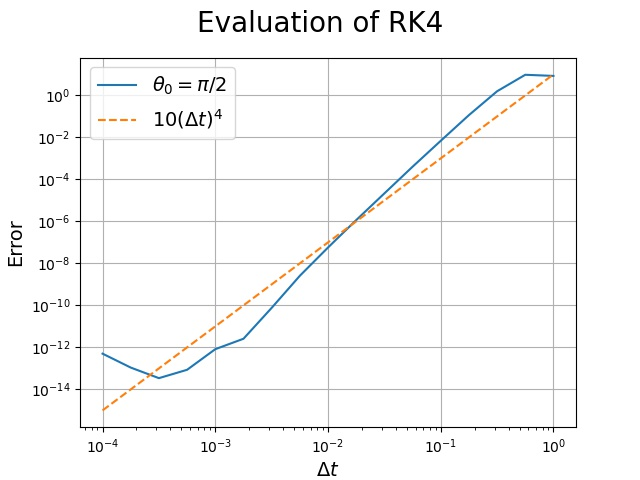
\includegraphics[scale=0.8]{figure/RK41/evaluation1/pi2_2021-2-9-222927.jpeg}
    \caption{初角度\(\dfrac{\pi}{2}における力学的エネルギーの精度\)}
    \label{fig:RK41_eval1_1}
  \end{center}
\end{figure}
\begin{figure}[H]
  \begin{center}
    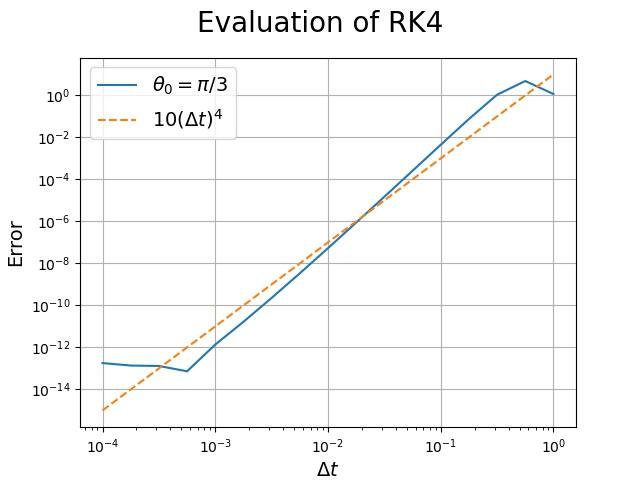
\includegraphics[scale=0.8]{figure/RK41/evaluation1/pi3_2021-2-9-222927.jpeg}
    \caption{初角度\(\dfrac{\pi}{3}における力学的エネルギーの精度\)}
    \label{fig:RK41_eval1_2}
  \end{center}
\end{figure}
\begin{figure}[H]
  \begin{center}
    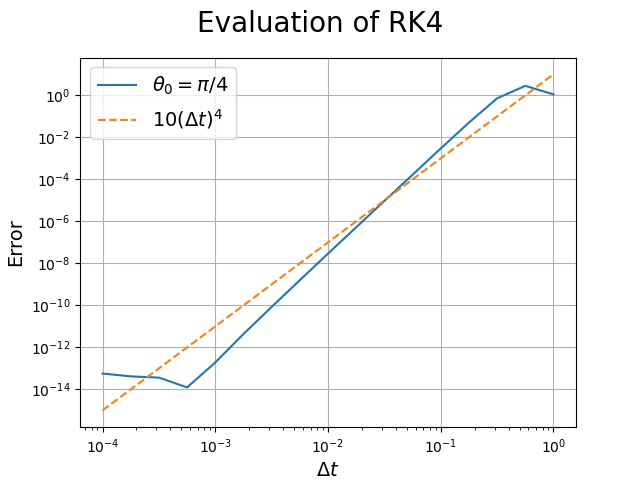
\includegraphics[scale=0.8]{figure/RK41/evaluation1/pi4_2021-2-9-222927.jpeg}
    \caption{初角度\(\dfrac{\pi}{4}における力学的エネルギーの精度\)}
    \label{fig:RK41_eval1_3}
  \end{center}
\end{figure}
\begin{figure}[H]
  \begin{center}
    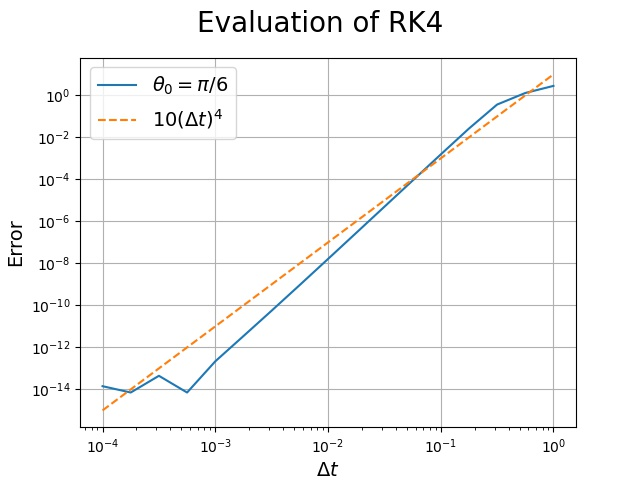
\includegraphics[scale=0.8]{figure/RK41/evaluation1/pi6_2021-2-9-222927.jpeg}
    \caption{初角度\(\dfrac{\pi}{6}における力学的エネルギーの精度\)}
    \label{fig:RK41_eval1_4}
  \end{center}
\end{figure}
\newpage
\subsection{考察} \label{ch:RK41_discussion}
まずアニメーションから読みとることのできる視覚的な情報についてであるが,ここからは運動のシミュレーションに不自然な点が特にないという事しか読み取ることができない.一方で振動の減衰などがはっきりと確認できるわけではないことから,系の力学的エネルギーがあまり変化していないのではないかという予想が立てられる.\par
次に,エネルギー誤差の時間変化についてである.\\
この図にひかれている点線は\(f(t) = 3\times10^{-9}t\)の補助線である.誤差は大域的にはこの直線に沿って増加し,局所的には振動している.ここに掲載した図\ref{fig:RK41_eval2}については初角度を\(\theta_0 = \dfrac{\pi}{4}\)としたものであるが,他の初角度に対しても同じような傾向(大域的には誤差が増加,局所的には振動)が確認できた.
振動しているように見える箇所は周期的に同じ形の変動を繰り返しているように見える.これは,それぞれの\(\theta\)について計算におけるエネルギーの減少しやすさや増加しやすさがある程度決まっており,そこを「周期的」に通るため同じような振動を繰り返しているように見えるのではないかと考えた.またそのように考えた場合,大域的に減少しているのは,「1周期」分の合計をとった時にその和が負の値であることによると考えられる(厳密な意味での周期的な運動ではないと考えられるため,「周期的」とあらわした).\par
最後に時間幅の変化に対する誤差の変化についてである.図\ref{fig:RK41_eval1_1}から図\ref{fig:RK41_eval1_4}の図中に記された点線は\(f(t) = 10(\Delta t)^{4}\)の補助線であり,4次の精度が達成されているかの目安となる.これらのグラフは両対数グラフになっていることに注意すると,この補助線よりも傾きが大きければ4次の精度を持っていると考えてよいと言える.\\
図より,どの初角度に対しても\(\Delta t = 10^0\)から\(\Delta t = 10^{-3}\)あたりにかけては4次の精度が成り立っている.一方で,\(\Delta t\)が\(10^{-3}\)よりも小さくなると誤差が増加傾向に転じる.これについて明確な理由はわかっていないが,上で述べたように,\(\theta\)に対応して誤差の変化のしやすさが決まっていると仮定し,\(\theta\)が大きい点(つまり角速度\(\omega\)が小さい点)における計算で誤差が広がりやすい場合を考えると,時間幅\(\Delta t\)が小さくなるにつれて\(\theta\)が大きい点で計算が実行される回数が増えていき,結果として一周期分の誤差増大量が大きくなると考えることができ辻褄が合う.\\
この仮定があっているかは,「1周期」分の計算においてどのような\(\theta\)で誤差が大きくなっているのかを確認すれば確かめられると考えたが,今回は時間不足で実施できなかった.また,このようなことが成り立つのであれば,誤差の増加が大きいと予想される\(\theta\)では時間幅\(\Delta t\)を大きくとるような可変的な時間幅を設定できるプログラムを作成することにより誤差の増加を緩やかにすることができるかもしれない.

\newpage
\section{二重振り子の運動}
この章では二重振り子の運動方程式に対してRunge-Kutta法を適用し,その特性を確認する.全体の流れとしては単振り子のときと同様である.
\subsection{二重振り子の運動方程式}
ここでは,長さ\(l_1\)で質点の質量が\(m_1\)の単振り子1と長さ\(l_2\)で質点の質量が\(m_2\)の単振り子2が連結された二重振り子を考える.鉛直下向きと単振り子1, 2がなす角をそれぞれ\(\theta_1, \theta_2\)とする.\\
このような二重振り子のLagrangianに対してEuler-Lagrange方程式を立てると以下のような運動方程式が求まる(導出の過程は\ref{ch:EL-eq}節に示した).なお,\(\phi = \theta_1-\theta_2\)とした.
\begin{subnumcases}
  {}
  \ddot{\theta_1} = \dfrac{-m_2l_2\dot{\theta_2}^2\sin{\phi}-(m_1+m_2)g\sin{\theta_1}-m_2l_1\dot{\theta_1}^2\sin{\phi}\cos{\phi}+m_2g\cos{\phi}\sin{\theta_2}}{(m_1+m_2)l_1-m_2l_1\cos^2{\phi}} & \\
  \ddot{\theta_2} = \dfrac{m_2l_2\dot{\theta_2}^2\cos{\phi}\sin{\phi}+(m_1+m_2)g\sin{\theta_1}\cos{\phi}+(m_1+m_2)l_1\dot{\theta_1}^2\sin{\phi}-(m_1+m_2)g\sin{\theta_2}}{(m_1+m_2)l_2-m_2l_2\cos^2{\phi}} &
\end{subnumcases}
これらの式において\(\omega_1 = \dot{\theta_1}\), \(\omega_2 = \dot{\theta_2}\)とすると以下のような連立一階微分方程式となる.\\
\begin{subnumcases}
  {\label{eom:double}}
  \dot{\theta_1} = \omega_1 & \\
  \ddot{\theta_1} = \dfrac{-m_2l_2\omega_2^2\sin{\phi}-(m_1+m_2)g\sin{\theta_1}-m_2l_1\omega_1^2\sin{\phi}\cos{\phi}+m_2g\cos{\phi}\sin{\theta_2}}{(m_1+m_2)l_1-m_2l_1\cos^2{\phi}} & \\
  \dot{\theta_2} = \omega_2 & \\
  \ddot{\theta_2} = \dfrac{m_2l_2\omega_2^2\cos{\phi}\sin{\phi}+(m_1+m_2)g\sin{\theta_1}\cos{\phi}+(m_1+m_2)l_1\omega_1^2\sin{\phi}-(m_1+m_2)g\sin{\theta_2}}{(m_1+m_2)l_2-m_2l_2\cos^2{\phi}} &
\end{subnumcases}
\subsection{二重振り子の運動方程式に対するRunge-Kutta法の適用}
\subsubsection{Runge-Kutta法の式について} \label{ch:RK42}
以下では式(\ref{eom:double})に対してRunge-Kutta法を適用することを考える.
\begin{equation}
  f(\theta_1, \theta_2, \omega_1, \omega_2) = \dfrac{-m_2l_2\omega_2^2\sin{\phi}-(m_1+m_2)g\sin{\theta_1}-m_2l_1\omega_1^2\sin{\phi}\cos{\phi}+m_2g\cos{\phi}\sin{\theta_2}}{(m_1+m_2)l_1-m_2l_1\cos^2{\phi}} \\
\end{equation}
\begin{equation}
  h(\theta_1, \theta_2, \omega_1, \omega_2) = \dfrac{m_2l_2\omega_2^2\cos{\phi}\sin{\phi}+(m_1+m_2)g\sin{\theta_1}\cos{\phi}+(m_1+m_2)l_1\omega_1^2\sin{\phi}-(m_1+m_2)g\sin{\theta_2}}{(m_1+m_2)l_2-m_2l_2\cos^2{\phi}}
\end{equation}
として,
\begin{gather}
  k_{11} = f(\theta_1^{(m)}, \theta_2^{(m)}, \omega_1^{(m)}, \omega_2^{(m)}) \\
  n_{11} = \omega_1^{(m)} \\
  k_{21} = h(\theta_1^{(m)}, \theta_2^{(m)}, \omega_1^{(m)}, \omega_2^{(m)}) \\
  n_{21} = \omega_2^{(m)} \\
  k_{12} = f\qty(\theta_1^{(m)}+n_{11}\dfrac{\Delta t}{2},\ \theta_2^{(m)}+n_{21}\dfrac{\Delta t}{2},\ \omega_1^{(m)}+k_{11}\dfrac{\Delta t}{2},\ \omega_2^{(m)}+k_{21}\dfrac{{\Delta t}}{2}) \\
  n_{12} = \omega_1^{(m)} + k_{11}\dfrac{\Delta t}{2} \\
  k_{22} = h\qty(\theta_1^{(m)}+n_{11}\dfrac{\Delta t}{2},\ \theta_2^{(m)}+n_{21}\dfrac{\Delta t}{2},\ \omega_1^{(m)}+k_{11}\dfrac{\Delta t}{2},\ \omega_2^{(m)}+k_{21}\dfrac{{\Delta t}}{2}) \\
  n_{22} = \omega_2^{(m)} + k_{21}\dfrac{\Delta t}{2} \\
  k_{13} = f\qty(\theta_1^{(m)}+n_{12}\dfrac{\Delta t}{2},\ \theta_2^{(m)}+n_{22}\dfrac{\Delta t}{2},\ \omega_1^{(m)}+k_{12}\dfrac{\Delta t}{2},\ \omega_2^{(m)}+k_{22}\dfrac{{\Delta t}}{2}) \\
  n_{13} = \omega_1^{(m)} + k_{12}\dfrac{\Delta t}{2} \\
  k_{23} = h\qty(\theta_1^{(m)}+n_{12}\dfrac{\Delta t}{2},\ \theta_2^{(m)}+n_{22}\dfrac{\Delta t}{2},\ \omega_1^{(m)}+k_{12}\dfrac{\Delta t}{2},\ \omega_2^{(m)}+k_{22}\dfrac{{\Delta t}}{2}) \\
  n_{23} = \omega_2^{(m)} + k_{22}\dfrac{\Delta t}{2} \\
  k_{14} = f\qty(\theta_1^{(m)}+n_{13}\Delta t,\ \theta_2^{(m)}+n_{23}\Delta t,\ \omega_1^{(m)}+k_{13}\Delta t,\ \omega_2^{(m)}+k_{23}\Delta t) \\
  n_{14} = \omega_1^{(m)} + k_{13}\Delta t \\
  k_{24} = f\qty(\theta_1^{(m)}+n_{13}\Delta t,\ \theta_2^{(m)}+n_{23}\Delta t,\ \omega_1^{(m)}+k_{13}\Delta t,\ \omega_2^{(m)}+k_{23}\Delta t) \\
  n_{24} = \omega_2^{(m)} + k_{23}\Delta t
\end{gather}
と定義すると,
\begin{equation}
  \omega_1^{(m+1)} = \omega_1^{(m)} + \qty(\dfrac{1}{6}k_{11}+\dfrac{1}{3}k_{12}+\dfrac{1}{3}k_{13}+\dfrac{1}{6}k_{14})\Delta t
\end{equation}
\begin{equation}
  \theta_1^{(m+1)} = \theta_1^{(m)} + \qty(\dfrac{1}{6}n_{11}+\dfrac{1}{3}n_{12}+\dfrac{1}{3}n_{13}+\dfrac{1}{6}n_{14})\Delta t
\end{equation}
\begin{equation}
  \omega_2^{(m+1)} = \omega_2^{(m)} + \qty(\dfrac{1}{6}k_{11}+\dfrac{1}{3}k_{12}+\dfrac{1}{3}k_{13}+\dfrac{1}{6}k_{14})\Delta t
\end{equation}
\begin{equation}
  \theta_2^{(m+1)} = \theta_2^{(m)} + \qty(\dfrac{1}{6}n_{21}+\dfrac{1}{3}n_{22}+\dfrac{1}{3}n_{23}+\dfrac{1}{6}n_{24})\Delta t
\end{equation}
と表せる.\\
単振り子と同様に,今回はこれをPythonによって実装し,運動の可視化およびそのエネルギー変化を可視化した.
運動の可視化のプログラムは付録中のソースコード\ref{src:RK42anim},エネルギーの時間変化のグラフを作成するプログラムはソースコード\ref{src:RK42eval2},時間幅の取り方によるエネルギーの誤差の変化を可視化するプログラムはソースコード\ref{src:RK42eval1}に示す.\\
\newpage
\subsubsection{Runge-Kutta法の妥当性について}
二重振り子の運動は\(\theta_1\),\ \(\theta_2\)が十分に小さいときのみ,近似を用いて解析解を求めることができる.したがって,微小角における解析解と数値解を比較することで,\ref{ch:RK42}節で定めたRunge-Kutta法の式による計算が妥当であるのかを確認することができる.\\
ここでは,簡単のために\(l = l_1 = l_2\)とし,\(\theta_1\),\ \(\theta_2 << 1\)である状況として\(\theta_1 = \theta_2 = 0.001\),\ \(\dot{\theta_1} = \dot{\theta_2} = 0\)と設定する.
このとき解析解は,
\begin{equation}
  \theta_1 = \dfrac{2-\sqrt{2}}{4000}\cos{(\sqrt{(2+\sqrt{2})\dfrac{g}{l}}t)} + \dfrac{2+\sqrt{2}}{4000}\cos{(\sqrt{(2-\sqrt{2})\dfrac{g}{l}}t)}
\end{equation}
\begin{equation}
  \theta_2 = -\dfrac{2\sqrt{2}-2}{4000}\cos{(\sqrt{(2+\sqrt{2})\dfrac{g}{l}}t)} + \dfrac{2\sqrt{2}+2}{4000}\cos{(\sqrt{(2-\sqrt{2})\dfrac{g}{l}}t)}
\end{equation}
と書くことができる.\\
Runge-Kutta法によって求まる数値解とこの解析解を比較するためのプログラムはソースコード\ref{src:RK42comp}に示した.
このコードを実行すると以下のようなグラフが得られる(ここでは特に\(l=1\)とした).
\begin{figure}[H]
  \begin{center}
    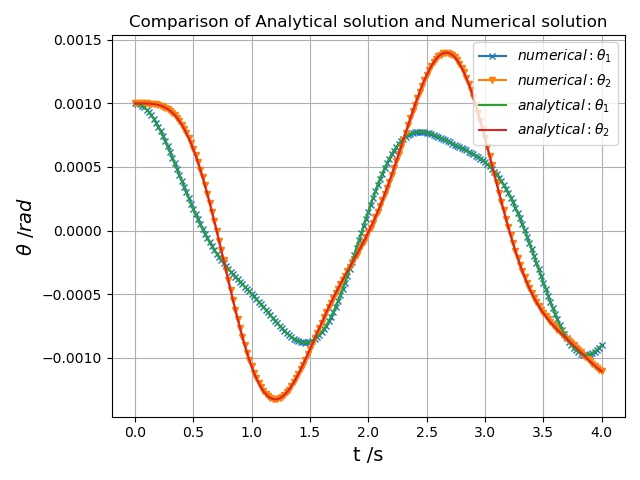
\includegraphics[scale=0.9]{figure/RK42/comparison1/2021-2-9-143754.jpeg}
    \caption{二重振り子の微小角近似における解析解とRK4による数値解の比較}
    \label{fig:RK42comp}
  \end{center}
\end{figure}
この図より,微小角近似における解析解とRunge-Kutta法による数値解は十分に一致しているため\ref{ch:RK42}節で定めた式が妥当であると考えることができる.
\newpage

\subsection{結果}

\subsubsection{二重振り子の運動のアニメーション}
ソースコード\ref{src:RK42anim}では長さ\(l_1,\ l_2\),質量\(m_1,\ m_2\),初角度\(\theta_{10},\ \theta_{20}\),初角速度\(\omega_{10},\ \omega_{20}\)がパラメータとして設定できるようになっているが,ここでは,\(l_1 = l_2 =1\),\ \(m_1 = m_2 =1\),\ \(\omega_{10} = \omega{20} = 0\)として運動の様子を見る.\\
また,このプログラムでは運動の様子をシミュレーションしたアニメーションがgifファイルとして保存できるが,このレポート上にgifを直接掲載するのは難しかったため,以下のリンク先(Google drive)に保存した.
\begin{itemize}
  \item \href{https://drive.google.com/file/d/1MPjW_B_pwXl1CM5LKhAw7Za5CbDMDMm1/view?usp=sharing}{初角度\(\theta_{10} = \dfrac{\pi}{2},\ \theta_{20} = \dfrac{5\pi}{4}\)の二重振り子}
  \item \href{https://drive.google.com/file/d/1TJpUKRKpi0ewUbH6xrBYIEyFGCoGV60K/view?usp=sharing}{初角度\(\theta_{10} = \dfrac{\pi}{4},\ \theta_{20} = \dfrac{\pi}{3}\)の二重振り子}
  \item \href{https://drive.google.com/file/d/1aUWOTSOAlM5S7ICsEniOS-E7f1XcNfjs/view?usp=sharing}{初角度\(\theta_{10} = \dfrac{\pi}{2},\ \theta_{20} = \dfrac{\pi}{2}\)の二重振り子}
\end{itemize}

\newpage
\subsubsection{エネルギー誤差の時間変化}
この二重振り子の系では力学的エネルギーが保存されるが,Runge-Kutta法を用いて数値計算をした場合には単振り子の場合と同じように,系全体のエネルギーが保存されるとは限らない.そのため,ここではいくつかの初期条件に対して時間経過とともに系全体のエネルギーがどのように変化するのかをグラフにまとめる.\\
以下に示す図において,横軸はすべて時間を表し,左上のグラフは系全体のエネルギーの変化,右上のグラフは振り子1, 2の運動エネルギー(\(T_1,\ T_2\))とポテンシャルエネルギー(\(U_1,\ U_2\))の変化,左下のグラフは振り子1, 2の力学的エネルギー(\(H_1, H_2\))の変化,右下のグラフは,真の力学的エネルギーを\(E_0\),計算された力学的エネルギーを\(E\)としたときの,\(\log \left|1-\dfrac{E}{E_0}\right|\)の変化をそれぞれ表している.
なお,この図を作成するプログラムはソースコード\ref{src:RK42eval2}であり,パラメータとして\(l_1,\ l_2,\ m_1, m_2,\ \theta_{10},\ \theta_{20},\ \omega_{10},\ \omega_{20}\)を設定することができるが,以下に示す図では,\(l_1 = l_2 = 1.0\), \(m_1 = m_2 = 1.0\), \(\omega_{10} = \omega_{20} = 0\)と固定している.
\begin{figure}[H]
  \begin{center}
    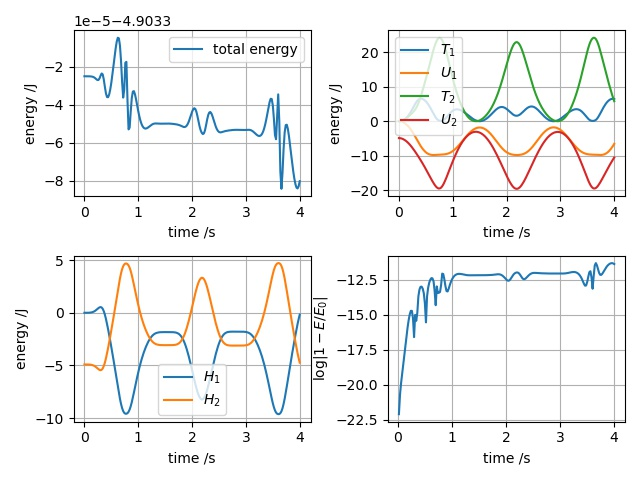
\includegraphics{figure/RK42/evaluation2/pi2_pi3_2021-2-9-132931.jpeg}
    \caption{\(\theta_{10} = \dfrac{\pi}{2},\ \theta_{20}  = \dfrac{\pi}{3}\)のときのエネルギーの時間変化}
    \label{fig:RK42-eval2-pi2-pi3}
  \end{center}
\end{figure}
\begin{figure}[H]
  \begin{center}
    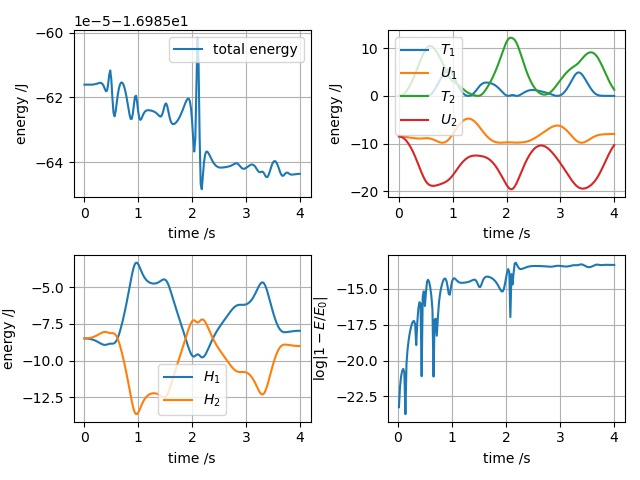
\includegraphics{figure/RK42/evaluation2/pi6_pi2_2021-2-9-13308.jpeg}
    \caption{\(\theta_{10} = \dfrac{\pi}{6},\ \theta_{20}  = \dfrac{\pi}{3}\)のときのエネルギーの時間変化}
    \label{fig:RK42-eval2-pi6-pi3}
  \end{center}
\end{figure}
これらの図を見ると,系全体のエネルギーは計算の誤差により\(10^{-5}\)のオーダーで減少していっていることがわかる.

\newpage
\subsubsection{時間幅の取り方による誤差の変化}
ここでは単振り子の場合と同じようにRunge-Kutta法における時間幅\(\Delta t\)の取り方によってエネルギーの誤差がどのように変化しているかを確認する.\\
以下に示す図\ref{fig:RK42-eval1-pi2-pi3}から図\ref{fig:RK42-eval1-pi6-pi3}はソースコード\ref{src:RK42eval1}において,\(l_1=l_2=1.0\),\ \(m_1=m_2=1.0\),\ \(\omega_{10}=\omega_{20}=0\)としたうえで初角度をそれぞれ\(\theta_{10} = \dfrac{\pi}{2},\ \theta_{20}  = \dfrac{\pi}{3}\), \(\theta_{10} = \dfrac{\pi}{6},\ \theta_{20}  = \dfrac{\pi}{3}\)と設定して得られたグラフである.なお,ここでの誤差は4秒経過後の\(|E-E_0|\)と定義した.\\
\begin{figure}[H]
  \begin{center}
    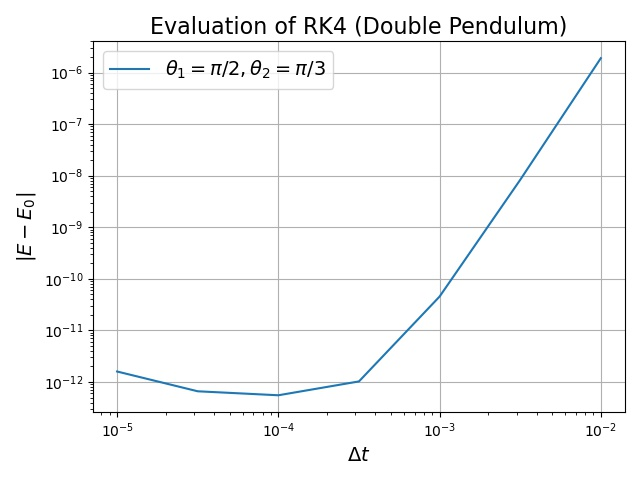
\includegraphics{figure/RK42/evaluation1/pi2_pi3_2021-2-9-135446.jpeg}
    \caption{\(\theta_{10} = \dfrac{\pi}{2},\ \theta_{20}  = \dfrac{\pi}{3}\)としたときのRK4の次数}
    \label{fig:RK42-eval1-pi2-pi3}
  \end{center}
\end{figure}
\begin{figure}[H]
  \begin{center}
    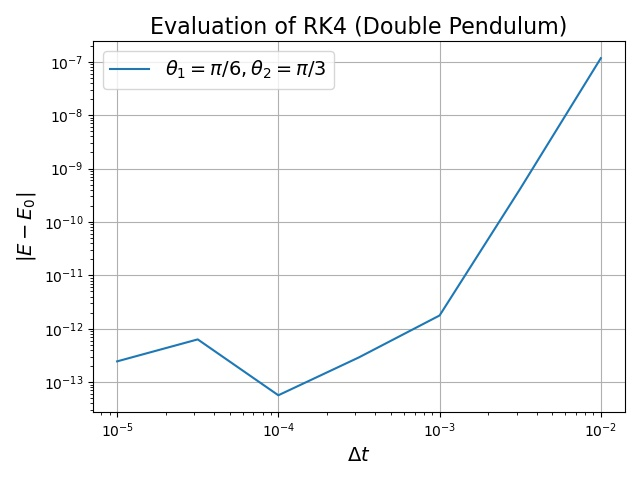
\includegraphics{figure/RK42/evaluation1/pi6_pi3_2021-2-9-135446.jpeg}
    \caption{\(\theta_{10} = \dfrac{\pi}{6},\ \theta_{20}  = \dfrac{\pi}{3}\)としたときのRK4の次数}
    \label{fig:RK42-eval1-pi6-pi3}
  \end{center}
\end{figure}
これらの図を見て言えることとしては,\( 10^{-3} \leq \Delta t \leq 10^{-2}\)の範囲では期待される4次の精度が出ているが,それよりも\(\Delta t\)を小さくとると4次の精度を達成しているとはいえないということである.これは,ここに示した初角度の設定に限定されるものではなく,ほかの初角度の組み合わせにおいても全体的に同じ傾向が見られた.

\newpage
\subsection{考察}
まずアニメーションについてであるが,二重振り子はカオス運動を起こすということから人間が簡単に予想できるほど単純な動きはせずこのアニメーションが正しく現実の二重振り子を再現できているかは判断することができない.強いて言うとするならば,質点の位置が連続的に変化していることは確かめられるため,Runge-Kutta法の計算が正しく実行されていると推測できる.\par
次に,系全体のエネルギーが時間経過とともにどのように変化するかについてであるが,これについては単振り子の場合と同じように,時間経過とともに計算される系全体のエネルギーは小さくなっていき正しい値からは離れていくという結果が得られた.大域的に見たときはエネルギーが減少しているということは単振り子の場合と共通しているが,一方で局所的に見たときのエネルギー変化については相違点がある.単振り子ではエネルギーの変化が単純な振動をしているように捉えることができたが,二重振り子では少し複雑な振動を繰り返しているように見える.\\
これは単振り子では角度\(\theta\)と角速度\(\omega\)が単純なトレードオフ関係にあったことに対し,二重振り子ではそうではないということによるのではないかと考えた.これはこの後述べる誤差の\(\Delta t\)依存性の議論にも共通する点である.\par
最後に,誤差の\(\Delta t\)依存性についてである.\(\Delta t\)を小さくとりすぎると誤差が大きくなってしまうという現象は単振り子の場合にも共通しており,これらの運動に対してRunge-Kutta法を適用したときの性質には類似性があると考えられる.単振り子でこのような傾向があることの理由として\ref{ch:RK41_discussion}節では,誤差の広がりやすさが\(\theta\)に依存しており,\(\Delta t\)を小さくすると誤差が広がりやすい\(\theta\)の近傍での計算回数が増えるためではないかということを述べた.\\
二重振り子の場合についても単振り子の場合と同じように誤差の広がり方がある程度\(\theta\)に依存するのであれば,このような現象は説明できると考えられる.しかし,二重振り子は単振り子ほど運動が単純ではないため,単振り子と二重振り子を簡単に比較することは望ましくない.特に,単振り子では\(\theta\)が大きいならば\(\omega\)が小さいということが力学的エネルギー保存則から簡単に言えたが,二重振り子については片方の振り子に注目したとき,\(\theta\)が大きく,かつ\(\omega\)も大きいという状況がありうるので単振り子ほど単純な説明ができるとは限らない.\\
これを確かめるためには誤差の広がり方の\(\theta\)および\(\omega\)に対する依存性を確かめるプログラムを作成すればよいと考えられるが,今回は時間不足のため確認できなかった.\par
今回新たに生まれた疑問に関しては明確な理由を述べることができなかったが,はじめに述べた目的である「系全体のエネルギーがRunge-Kutta法によってどれくらい保存されるのか」を確かめるということについては\(\Delta t = 10^{-3}\)程度までは4次の精度をもち,\(\Delta t =10^{-3}\)程度とすれば単振り子・二重振り子いずれの場合についてもエネルギーの誤差は\(10^{-10}\)以下まで抑えることができると分かった.
\newpage
\section{付録}
\subsection{二重振り子の運動方程式の導出} \label{ch:EL-eq}
長さ\(l_1\),質量\(m_1\)の振り子の下に長さ\(l_2\), 質量\(m_2\)の振り子を連結した二重振り子を考える.\\
振り子1, 2が鉛直下向きとなす角を\(\theta_1,\ \theta_2\)としてデカルト座標で表すと,
\begin{equation}
  (x_1,\ y_1) = (l_1\sin{\theta_1},\ -l_1\cos{\theta_1})
\end{equation}
\begin{equation}
  (x_2,\ y_2) = (l_1\sin{\theta_1} + l_2\sin{\theta_2},\ -l_1\cos{\theta_1}-l_2\cos{\theta_2})
\end{equation}
となり,これを時間微分すると,
\begin{equation}
  (\dot{x_1},\ \dot{y_1}) = (l_1\dot{\theta_1}\cos{\theta_1},\ l_1\dot{\theta_1}\sin{\theta_1})
\end{equation}
\begin{equation}
  (\dot{x_2},\ \dot{y_2}) = (l_1\dot{\theta_1}\cos{\theta_1} + l_2\dot{\theta_2}\cos{\theta_2},\ l_1\dot{\theta_1}\sin{\theta_1}+l_2\dot{\theta_2}\sin{\theta_2})
\end{equation}
となる.\\
ふりこ\(i\)の運動エネルギー,ポテンシャルエネルギーをそれぞれ\(T_i,\ U_i\)と表すとこの系のLagrangianは,
\begin{gather}
  \begin{split}
    L &= T_1 + T_2 - U_1 -U_2 \\
      &= \dfrac{1}{2}m_1(\dot{x_1}^2+\dot{y_1}^2) + \dfrac{1}{2}m_2(\dot{x_2}^2+\dot{y_2}^2) -m_1gy_1 -m_2gy_2 \\
      &= \dfrac{1}{2}m_1l_1^2\dot{\theta_1}^2 + \dfrac{1}{2}m_2\qty[l_1^2\dot{\theta_1}^2+l_2^2\dot{\theta_2}^2+2l_1l_2\dot{\theta_1}\dot{\theta_2}\cos\phi]+m_1gl_1\cos{\theta_1}+m_2g(l_1\cos{\theta_1+l_2\cos{\theta_2}})
  \end{split}
\end{gather}
となる.ただし\(\theta_1-\theta_2 = \phi\)とした.これをEuler-Lagrange方程式に代入すると,
\begin{equation}
  \begin{pmatrix}
    (m_1+m_2)l_1 & m_2l_2\cos{\phi} \\
    l_1\cos{\phi} & l_2 \\
  \end{pmatrix}
  \mqty(\ddot{\theta_1} \\ \ddot{\theta_2})
  =
  \mqty(-m_2l_2\dot{\theta_2}^2\sin{\phi}-(m_1+m_2)g\sin{\theta_1} \\ l_1\dot{\theta_1}^2\sin{\phi}-g\sin{\theta_2})
\end{equation}
が求まる.ここで,
\begin{equation}
  \mqty((m_1+m_2)l_1 & m_2l_2\cos{\phi} \\ l_1\cos{\phi} & l_2)^{-1} \\= \dfrac{1}{(m_1+m_2)l_1l_2-m_2l_1l_2\cos^2{\phi}}\mqty(l_2 & -m_2l_2\cos{\phi} \\ -l_1\cos{\phi} & (m_1+m_2)l_1)
\end{equation}
であることから,
\begin{subnumcases}
  {}
  \ddot{\theta_1} = \dfrac{-m_2l_2\dot{\theta_2}^2\sin{\phi}-(m_1+m_2)g\sin{\theta_1}-m_2l_1\dot{\theta_1}^2\sin{\phi}\cos{\phi}+m_2g\cos{\phi}\sin{\theta_2}}{(m_1+m_2)l_1-m_2l_1\cos^2{\phi}} & \\
  \ddot{\theta_2} = \dfrac{m_2l_2\dot{\theta_2}^2\cos{\phi}\sin{\phi}+(m_1+m_2)g\sin{\theta_1}\cos{\phi}+(m_1+m_2)l_1\dot{\theta_1}^2\sin{\phi}-(m_1+m_2)g\sin{\theta_2}}{(m_1+m_2)l_2-m_2l_2\cos^2{\phi}} &
\end{subnumcases}
が求まる.

\newpage
\subsection{計算機環境}
\begin{itemize}
  \item CPU: Intel(R) Core(TM) i7-9700K CPU @ 3.60GHz   3.60 GHz
  \item メモリ: 16.0 GB
  \item OS: Windows10 Home
  \item プログラミング言語: Python 3.8.5
\end{itemize}
\newpage
\subsection{ソースコード}
\lstinputlisting[caption=単振り子のアニメーション作成, label=src:RK41anim]{RK41_animation.py}
\newpage
\lstinputlisting[caption=単振り子のエネルギーの時間変化について, label=src:RK41eval2]{RK41_evaluation2.py}
\newpage
\lstinputlisting[caption=単振り子におけるRK4の次数について, label=src:RK41eval1]{RK41_evaluation1.py}
\newpage
\lstinputlisting[caption=二重振り子における微小角近似の解析解とRk4の比較, label=src:RK42comp]{RK42_comparison1.py}
\newpage
\lstinputlisting[caption=二重振り子のアニメーション作成, label=src:RK42anim]{RK42_animation.py}
\newpage
\lstinputlisting[caption=二重振り子のエネルギーの時間変化について, label=src:RK42eval2]{RK42_evaluation2.py}
\newpage
\lstinputlisting[caption=二重振り子におけるRK4の次数について, label=src:RK42eval1]{RK42_evaluation1.py}
\newpage
\subsection{参考文献}
\begin{itemize}
  \item 畑浩之 「基幹講座 物理学 解析力学」 東京図書
\end{itemize}
\end{document}